\documentclass[10pt,a4paper]{article}
\usepackage{amsmath,amsfonts,amsthm,amssymb}
\usepackage{verbatim}
\usepackage{setspace}
\usepackage{fancyhdr}
\usepackage{lastpage}
\usepackage[colorlinks]{hyperref}
\usepackage{extramarks}
\usepackage{chngpage}
\usepackage{soul,color}
\usepackage{enumerate}
\usepackage{graphicx,float,wrapfig}
\usepackage{subfig}
\usepackage{listings}
\usepackage{xltxtra}
\usepackage{xeCJK}
\usepackage{xunicode}
\usepackage{fontspec}

\newcommand{\Class}{数据库系统概论}
\newcommand{\ClassInstructor}{冯建华\ 马冬哲}
\newcommand{\Title}{大作业}
\newcommand{\DueDate}{2012.1.13}
\newcommand{\StudentName}{肖桐\ 毛佳昕\ 褥震\ 金旻俊}
\newcommand{\StudentClass}{Group30\ \ 计92}
\newcommand{\StudentNumber}{}

\setCJKmainfont[Mapping=tex-text]{Microsoft YaHei}
\punctstyle{quanjiao}

% In case you need to adjust margins:
\topmargin=-0.45in      %
\evensidemargin=0in     %
\oddsidemargin=0in      %
\textwidth=6.5in        %
\textheight=9.0in       %
\headsep=0.25in         %

% Setup the header and footer
\pagestyle{fancy}                                                       %
\lhead{\StudentName}                                                 %
\chead{\Title}  %
\rhead{\firstxmark}                                                     %
\lfoot{\lastxmark}                                                      %
\cfoot{}                                                                %
\rfoot{Page\ \thepage\ of\ \protect\pageref{LastPage}}                          %
\renewcommand\headrulewidth{0.4pt}                                      %
\renewcommand\footrulewidth{0.4pt}                                      %

%%%%%%%%%%%%%%%%%%%%%%%%%%%%%%%%%%%%%%%%%%%%%%%%%%%%%%%%%%%%%
% Some tools
\newcommand{\enterProblemHeader}[1]{\nobreak\extramarks{#1}{#1 continued on next page\ldots}\nobreak%
                                    \nobreak\extramarks{#1 (continued)}{#1 continued on next page\ldots}\nobreak}%
\newcommand{\exitProblemHeader}[1]{\nobreak\extramarks{#1 (continued)}{#1 continued on next page\ldots}\nobreak%
                                   \nobreak\extramarks{#1}{}\nobreak}%

\newcommand{\homeworkProblemName}{}%
\newcounter{homeworkProblemCounter}%
\newenvironment{homeworkProblem}[1][Problem \arabic{homeworkProblemCounter}]%
  {\stepcounter{homeworkProblemCounter}%
   \renewcommand{\homeworkProblemName}{#1}%
   \section*{\homeworkProblemName}%
   \enterProblemHeader{\homeworkProblemName}}%
  {\exitProblemHeader{\homeworkProblemName}}%

\newcommand{\homeworkSectionName}{}%
\newlength{\homeworkSectionLabelLength}{}%
\newenvironment{homeworkSection}[1]%
  {% We put this space here to make sure we're not connected to the above.

   \renewcommand{\homeworkSectionName}{#1}%
   \settowidth{\homeworkSectionLabelLength}{\homeworkSectionName}%
   \addtolength{\homeworkSectionLabelLength}{0.25in}%
   \changetext{}{-\homeworkSectionLabelLength}{}{}{}%
   \subsection*{\homeworkSectionName}%
   \enterProblemHeader{\homeworkProblemName\ [\homeworkSectionName]}}%
  {\enterProblemHeader{\homeworkProblemName}%

   % We put the blank space above in order to make sure this margin
   % change doesn't happen too soon.
   \changetext{}{+\homeworkSectionLabelLength}{}{}{}}%

\newcommand{\Answer}{\ \\\textbf{解答:} }
\newcommand{\Acknowledgement}[1]{\ \\{\bf 感谢:} #1}

%%%%%%%%%%%%%%%%%%%%%%%%%%%%%%%%%%%%%%%%%%%%%%%%%%%%%%%%%%%%%


%%%%%%%%%%%%%%%%%%%%%%%%%%%%%%%%%%%%%%%%%%%%%%%%%%%%%%%%%%%%%
% Make title
\title{\textmd{\bf \Class: \Title}\\{\large 授课教师: \textit{\ClassInstructor}}\\\normalsize\vspace{0.1in}\small{截至日期: \DueDate}}
\date{}
\author{\StudentClass\ \ \StudentName}
%%%%%%%%%%%%%%%%%%%%%%%%%%%%%%%%%%%%%%%%%%%%%%%%%%%%%%%%%%%%%

\begin{document}
\begin{spacing}{1.1}
\maketitle \thispagestyle{empty}

%%%%%%%%%%%%%%%%%%%%%%%%%%%%%%%%%%%%%%%%%%%%%%%%%%

\begin{homeworkProblem}[整体框架]
整个工程主要由以下四部分组成,可以用图~\ref{fig-frame}来表示整体的框架。
\begin{enumerate}
\item \textbf{Column类}\\[5pt]
对于数据库的每个列信息的一个封装,包括列名、类型、索引等信息,以及根据索引做屏蔽等函数。
\item \textbf{Table类}\\[5pt]
对与数据库的每个表信息的一个封装,包括表名、每行的信息、每列的信息,以及给定条件做筛选等函数。
\item \textbf{SQLParser类}\\[5pt]
用于SQL语句解析的类,提取需要的信息。
\item \textbf{Executor类}\\[5pt]
实现逻辑控制的类,执行client里面应做的事情。
\end{enumerate}
\begin{figure}[h!]
\centering
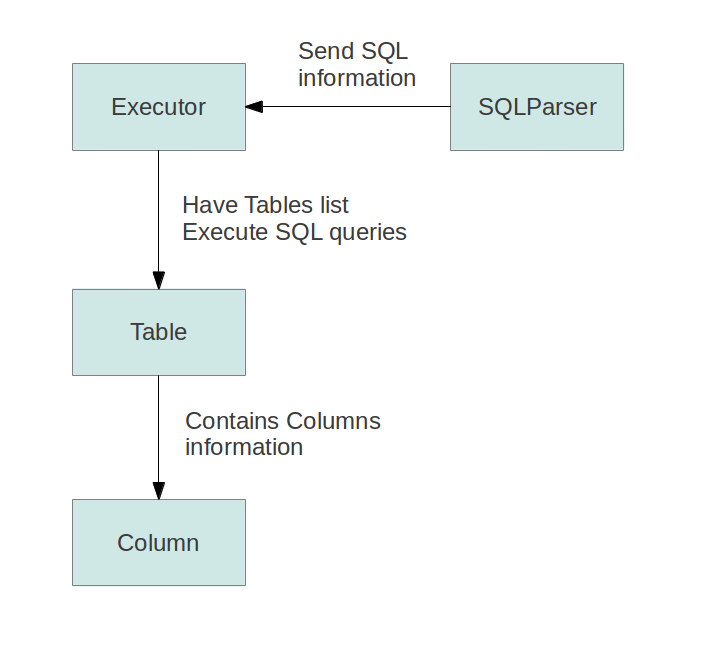
\includegraphics[width=0.5\textwidth]{frame.png}
\caption{工程整体框架示意图}
\label{fig-frame}
\end{figure}
\end{homeworkProblem}

\begin{homeworkProblem}[数据存储机制]
\begin{enumerate}
\item \textbf{行内容存储}\\[5pt]
我们组采用了kyotocabinet的TreeDB来管理数据库每行内容的存储,为方便定位查找,每行的信息以定长的字节串的形式存储。每个整型的列,用4字节来表示其值;每个字符串型的列,用其声明长度加1来记录(加1是为了在末尾加入字符串结束符),长度不足的话,其结束符之后的字节随意填充。例如,对于这样的一个表:
\begin{verbatim}
tableA
colA    INTEGER
colB    VARCHAR(5)
colC    INTEGER
\end{verbatim}
若加入这样一行
\begin{verbatim}
255,'abcde',1
\end{verbatim}
则存入的记录如下,其中整数是以小端的形式存储的
\begin{center}
\begin{tabular}{|c|c|c|c|c|c|c|c|c|c|c|c|c|c|c|}
\hline
ff & 00 & 00 & 00 & 'a' & 'b' & 'c' & 'd' & 'e' & '$\backslash$0' & 80 & 00 & 00 & 00\\
\hline
\end{tabular}
\end{center}
\item \textbf{索引存储}\\[5pt]
此外,我们会对在train中出现在条件中的列做索引,原本索引是用HashDB来管理的,但由于其效率实在难以忍受,后来改为都存入内存中,用multimap作索引。我们对于每行用其行号作为唯一的隐藏主键。在load和insert时,即会对每一行需要做索引的列添加索引。
\end{enumerate}
\end{homeworkProblem}

\begin{homeworkProblem}[查询的算法]
\begin{enumerate}
\item 解析SQL的SELECT语句,计算出所需要的行列信息。
\item 每个SELECT语句都可以表示为若干个表的join,这可以用一棵树表示,同时对每个节点会有一些限制条件。根据上一步得出的行列信息构建这样一棵树。
\item 计算出一个join的顺序,即给出一个树的遍历顺序。这里用到了一个简单的估价,对于每个节点估计符合其限制条件的行数。对于形如“colA = 1”这样的条件,估价函数为$\displaystyle \frac{totalRows}{diff\ keys}$;对于形如“colA < 100”这样的条件,估价函数为$\displaystyle totalRows\frac{key-minKey}{maxKey-minKey}$。估价越低,join的顺序越靠前。
\item 根据生成的join顺序依次做join。join的中间结果保存的是每个表符合条件的行号,每次join先对要join的表用其限制条件做筛选,返回一个集合。然后枚举中间结果,用值去找要join进来的表的索引,又得到一个集合。两集合的交即加入中间结果中。
\item 我们经过一些实验,对某个表做筛选采用了如下的方法。用上面提到过的估价函数对限制条件做从小到大的排序,然后取出第一个,利用索引得到满足条件的行号。接下来对于每行,从原表中取出行的内容,依次判断是否符合剩下的限制条件。如果都满足,则加入筛选结果中。
\end{enumerate}
\begin{figure}[h!]
\centering
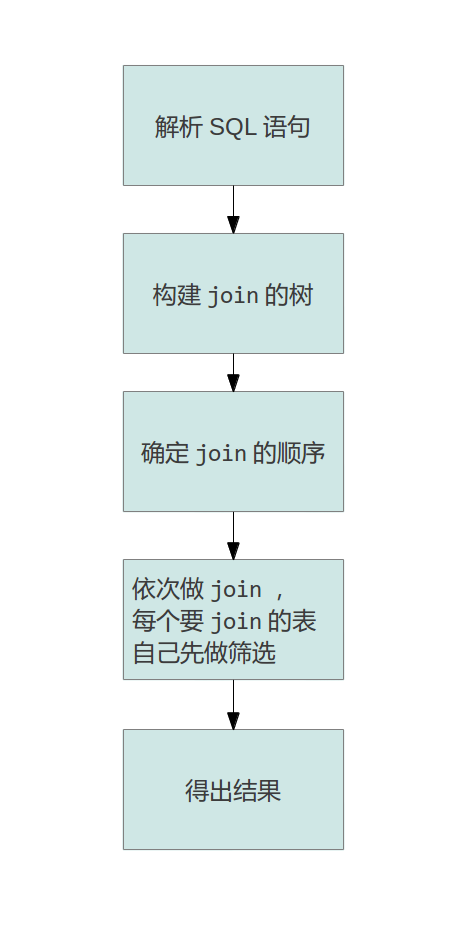
\includegraphics[width=0.3\textwidth]{join.png}
\caption{查询的算法流程}
\label{fig-join}
\end{figure}
\end{homeworkProblem}

\begin{homeworkProblem}[其他]
\begin{enumerate}
\item 参考书籍:数据库系统与实现,Hector Garcia-Molina, Jeffrey D. Ullman, Jennifer Widom。
\item 分工情况
\begin{center}
\begin{tabular}{|c|c|}
\hline
\multicolumn{2}{|c|}{\textbf{小组成员贡献率}}\\
\hline
肖桐 & 30\%\\
\hline
毛佳昕 & 30\%\\
\hline
褥震 & 20\%\\
\hline
金旻俊 & 20\%\\
\hline
\end{tabular}
\end{center}
\item 一些建议:如果可以的话,明年的大作业希望做成一个类似oj的形式,这样可能会给教学双方都减少些压力。
\end{enumerate}
\end{homeworkProblem}


%%%%%%%%%%%%%%%%%%%%%%%%%%%%%%%%%%%%%%%%%%%%%%%%%%

\end{spacing}
\end{document}
